\documentclass{standalone}
\usepackage{tikz}
\usetikzlibrary{arrows,decorations.markings,calc,positioning}

% "Add arrows to a smooth tikz function"
% from http://tex.stackexchange.com/a/163695
\tikzset{
   set arrow inside/.code={\pgfqkeys{/tikz/arrow inside}{#1}},
   set arrow inside={end/.initial=>, opt/.initial=},
   /pgf/decoration/Mark/.style={
      mark/.expanded=at position #1 with
      {
         \noexpand\arrow[\pgfkeysvalueof{/tikz/arrow inside/opt}]{\pgfkeysvalueof{/tikz/arrow inside/end}}
      }
   },
   arrow inside/.style 2 args={
      set arrow inside={#1},
      postaction={
         decorate,decoration={
            markings,Mark/.list={#2}
         }
      }
   },
}

\begin{document}
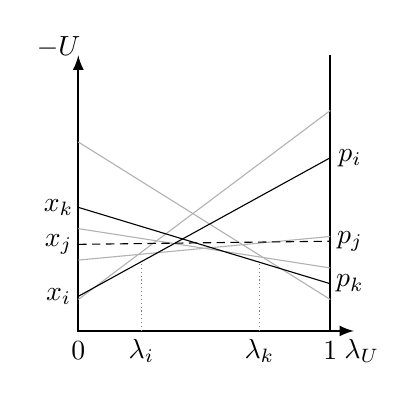
\begin{tikzpicture}



%\node[circle,fill=black,inner sep=0.05cm] (a3) at (1.11,1.45) {};
%\node[below left=-0.15cm of a3] {$A_3(\eta)$};

% axes
\draw[thick] (3.2,0) -- (3.2,3.5);
\draw[thick,latex-latex] (3.5,0) -- (0,0) -- (0,3.5);

%\node[black!50,font=\small,circle,fill=white,inner sep=0pt]
%   (lam1) at (2.7,-0.1) {$\lambda_1$};
%\draw[black!50,->] (lam1) -- (2.9,0.28);

%\node[black!50,font=\small,circle,fill=white,inner sep=0pt]
%   (lam2) at (-0.1,1.8) {$\lambda_2$};
%\draw[black!50,->] (lam2) -- (0.28,2.0);

% vertical lambda lines
\draw[black!50,densely dotted] (0.8,0.0) -- (0.8,0.88);
\draw[black!50,densely dotted] (2.3,0.0) -- (2.3,0.872);

% background slopes
\draw[black!30] (0.0,2.4) -- (3.2,0.4); % point B
\draw[black!30] (0.0,1.3) -- (3.2,0.8); % point C (p=0.8 x=1.3)
\draw[black!30] (0.0,0.9) -- (3.2,1.2); % point E (p=1.2 x=0.9)
\draw[black!30] (0.0,0.4) -- (3.2,2.8); % point F (p=2.8 x=0.4)

% slopes
\draw[black] (0.0,0.44) -- (3.2,2.2); % x_i, p_i
\draw[black,densely dashed] (0.0,1.1) -- (3.2,1.14); % x_j, p_j
\draw[black] (0.0,1.57) -- (3.2,0.6); % x_k, p_k

\node at (0.0,-0.25) {$0$};
\node at (3.2,-0.25) {$1$};
\node at (3.6,-0.25) {$\lambda_U$};

\node at (3.45,2.2) {$p_i$};
\node at (-0.25,0.44) {$x_i$};

\node at (3.45,1.14) {$p_j$};
\node at (-0.25,1.1) {$x_j$};

\node at (3.45,0.6) {$p_k$};
\node at (-0.25,1.57) {$x_k$};

\node at (-0.25,3.6) {$-U$};

\node at (0.8,-0.25) {$\lambda_i$};
\node at (2.3,-0.25) {$\lambda_k$};


\end{tikzpicture}
\end{document}
